\chapter{\textbf{Problem Formulation}}
This chapter describes different mathematical models we propose for user-managed SFC orchestration in MEC and show how our problem can be formulated as a constrained optimization problem. Specifically, Section \ref{section: system model} presents the system model, network model, and service model in user-managed SFC orchestration. Section \ref{section: formulation} shows the mathematical formulation of the User-managed Edge-enabled Chain orchestration Problem as constrained optimization.


\section{System Model}
\label{section: system model}
In this section, we describe our model.
Our model is able to represent existing edge-enabled architectures with required elements for bandwidth and processing resource allocation.
We adopt a time-slotted model and use $\mc{T}=\{0,\dots,T\}$ to denote the considered time horizon. Each timeslot $t\in\mc{T}$ represents a resource allocation phase with the duration of $\Theta$ seconds.   
In addition, we assume that our system is a user-managed system where each user receives light-weight feedback about the system operation, and is responsible for managing and resource allocation of service individually with the help of the feedback.
This system operation scheme keeps the system complexity and scale at a smaller scale, which enables us to achieve better solutions in section~\ref{chapter: Proposed Method}.  

\begin{figure}
	\centering
	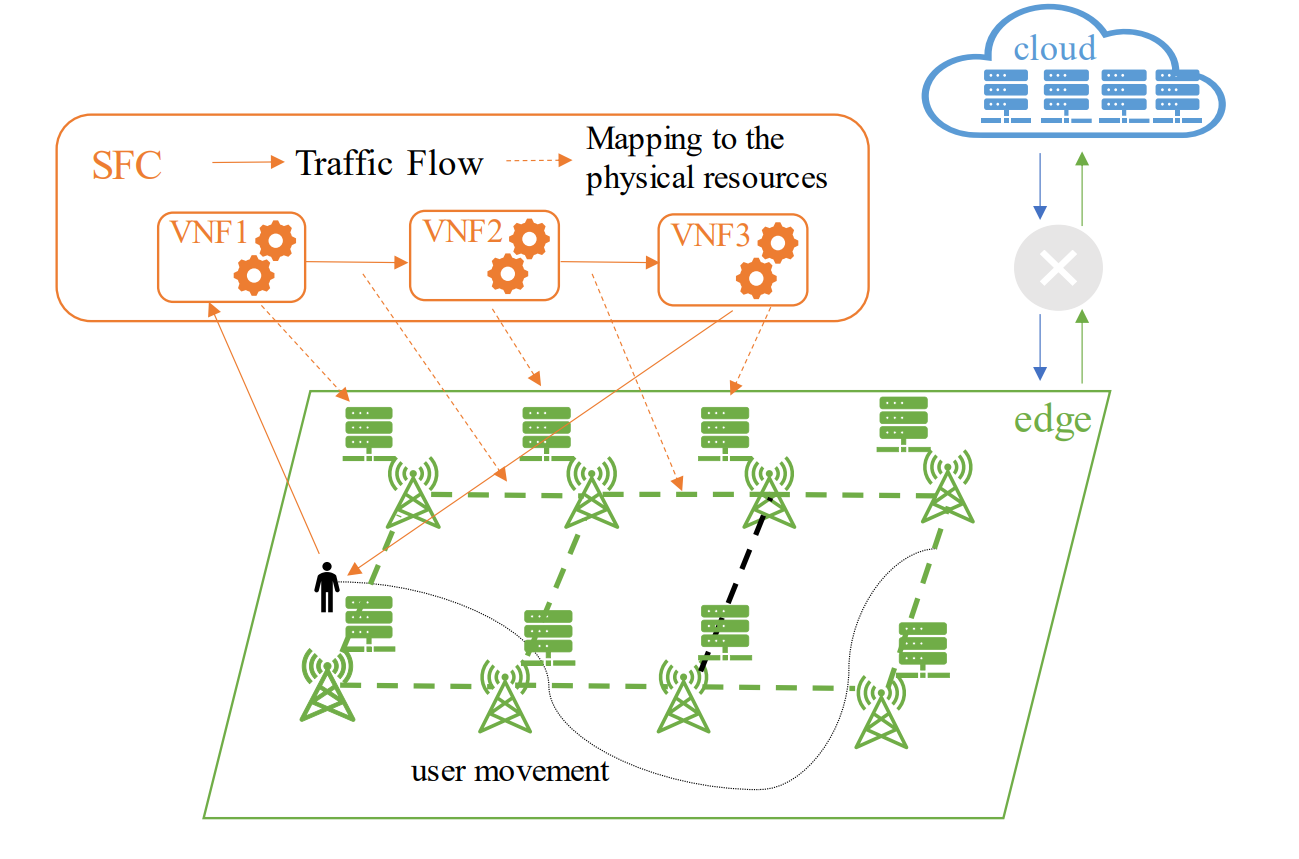
\includegraphics[width=0.9\linewidth]{figs/MEC_SFCdiagram_colored2.PNG}
		\vspace{\baselineskip}
	\caption{An example of SFC placement in MEC}
	\label{fig:mecsfcdiagram}
\end{figure}
\subsection{Network Model}
As illustrated in figure \ref{fig:mecsfcdiagram}, We consider a remote cloud $C$ and a mobile access network consisting of a set of base stations, each of which is bridged with an edge server, and is accessible through wireless channels.
Each base station is equipped with an edge server, where the set of all edge servers is denoted by $\mc{E}$. The cumulative processing capacity of the cloud and each edge server $e\in\mc{E}$ (in terms of the number of CPU cores) in timeslot $t$ is denoted, respectively, by $c_{C}(t)$ and $c_{e}(t)$\footnote{When cores are heterogeneous we must normalize the numbers with regard to the weakest CPU core in the system}. Edge servers are connected to each other and the remote cloud through a capacitated backbone network $G(\mc{R}, \mc{L})$, where $\mc{R}$ is the set of backbone routers and $\mc{L}$ is the set of backbone links. At time $t$, each link $\ell\in\mc{L}$ is associated with the bandwidth capacity $b_{\ell}(t)$ and propagation delay $d_{\ell}(t)$. We also refer to a link by its two endpoints, \eg, $d_{a,b}$ is the delay of the link between $a$ and $b$. Generally, the delay between edge servers and the cloud is significantly higher than the delay between edge servers. While, propagation delay within the cloud is considered to be negligible. 

\subsection{Service Model}
\label{sec:SFCrequest}
We assume that each user who roams in the vicinity of the access network has a mobile device $u$  (\eg\ Smartphone, tablet, in-vehicle infotainment system) with the processing capacity of $c_{u}(t)$, which is always connected to the nearest base station (denoted by $\beta$). Each user in time slot $t$ generates traffic at rate $\lambda(t)$ megabits per-second (Mbps) and requires it to be processed by a set of pre-determined \emph{services} in strict order (\aka\ a service chain). Each service is a software program (\eg\ video transcoder, firewall, and logger) that can be deployed in the cloud or an edge server with the means of state-of-the art virtualization methods such as Container~\cite{containerNFV}. We use $\mc{S}=(s_1, \dots, s_K)$ to denote the list of the user-required services and assume that service $s_i$ incurs $\pi_{s_{i}}$ seconds of delay to process $1$ Mbps of incoming data by using $1$ unit of CPU core. Moreover, each service can scale the user input traffic by a factor of $\alpha_{s_i}\in[0,\infty)$ before sending it to the next service due to operations such as encoding or decoding. Consequently, the traffic rate to the service $s_{i}$ can be computed by,
\begin{gather}
	\lambda_{s_{i}}(t) = \lambda(t) \times \prod_{j=1}^{i-1} \alpha_{s_j}.
\end{gather}
Note that service migration is inevitable as the user moves in the environment. Let $\mc{N}=\mc{E}\cup\{C, u\}$ represent all nodes that can host a service and provide the required processing capacity. The \textit{migration delay} $\rho_{a, b}^{s_{i}}(t)$
is defined as the time that the user has to wait for if her service $s_{i}$ is migrated from the source node $a$ to the destination node $b$ ($a,b \in \mc{N}$) in timeslot $t$ (clearly, $\rho_{a, a}^{s_{i}}(t)=0$). To serve a user request, each service in $\mc{S}$ should be deployed in a node with sufficient processing capacity, and the network routing should be adjusted such that user traffic goes through the services in the specified order. Finally, we assume that there is a special service at the end of the chain which is constrained to be placed on the user device. This technique guarantees that the results of the computation is carried back to the user.  

\begin{table}[t]
	\ra{1.2}
	\centering
	\caption{List of main notations in \myproblem\ formulation}
	\begin{tabular}{ll}
		\toprule
		Notation & \multicolumn{1}{c}{Description} \\
		\midrule
		$\mc{T}$ & Time frame \\
		$\mc{E}$ &  Set of all edge servers\\
		$C$ &  Cloud \\
		$\mc{L}$ &  Set of backbone links\\
		$\mc{R}$ & Set of backbone routers\\
		$b_{\ell}(t)$ & Current bandwidth capacity on link $\ell$\\
		$d_{\ell} (t)$ & Current propagation delay on link $\ell$ \\
		$c_{n}(t)$ & Current CPU core of node $n$ \\
		$\beta (t)$ & Current connected base station \\
		$\mc{S}$ & Set of all available services \\
		$\mc{N}$ & Set of all selectable nodes\\
		$\lambda(t)$ & Current user traffic rate \\
		$\pi_{s}$ & Processing delay factor of service $s$ \\
		$\alpha_{s}$ & Traffic scale factor of service $s$ \\
		$\rho_{a, b}^{s}(t)$ & Migration delay of service $s$ from node $a$ to node $b$ \\
		$\delta^{+}(r), \delta^{-}(r)$ & Incoming and outgoing links of router $r$\\
		%$\mc{C(t)}$ & Context \\
		%$\mc{S}(t)$ & SFC at time slot $t$ \\
		$x^s_n(t)$ & Current placement of service $s$ on node $n$\\
		$y^{s_i}_\ell(t)$ & Usage of link $\ell$ to route traffic from service $s_i$ to $s_{i+1}$  \\
		
		\bottomrule
	\end{tabular}
	\label{tab:System parameter}
\end{table}



\section{Problem Formulation}
\label{section: formulation}
In this section, we formally define the problem of SFC orchestration at the edge. Specifically, We consider the problem of service placement, service migration, and traffic routing with the objective of minimizing the user-perceived end-to-end delay. 
%We assume that users receive sophisticated feedback and manage manage their own services individually. This system operation scheme keeps the system complexity and scale at a smaller scale which enables us to achieve better solutions in later section. We call this the User-managed Edge-enabled Chain Placement Problem (\ie\ \myproblem).

\cat{Placement} To specify the placement of a service chain, we define binary decision variables $x_{n}^{s}(t)$, where $x_{n}^{s}(t)=1$ means that service $s$ is placed on the node $n$ in time slot $t$. We use the following constraint to ensure that every service in the chain is placed on a node,
\begin{gather}
	\sum_{n\in\mc{N}} x_{n}^{s}(t) = 1. 
	\qquad 
	\forall s\in\mc{S}, t\in\mc{T}
\end{gather}
Recent studies show that co-locating a user's services compromises the system reliability~\cite{colocatingService}. Thus, we include the following constraint to prevent co-located services,
\begin{gather}
	\sum_{s\in\mc{S}} x_{n}^{s}(t) \le 1. 
	\qquad 
	\forall n\in\mc{N}, t\in\mc{T}
\end{gather}

\cat{Routing}
A single path consisting of intermediate links and routers with enough bandwidth should be provisioned for every consecutive services $s_{i}$ and $s_{i+1}$ that are placed on separate nodes. To this end, we define binary decision variables $y_{\ell}^{s_{i}}(t)$, where $y_{\ell}^{s_{i}}(t)=1$ means that link $\ell$ is used to route the traffic between hosting nodes of services $s_{i}$ and $s_{i+1}$. Additionally, to unify the formulation and present it in a compact manner, we assume that a base station is a router and also assume that a hypothetical router resides on the user hand-held device the connects the device to the corresponding base station. We call this hypothetical router $\beta^{'}$ and denote the extended set of router by $\mc{R}^{'}=\mc{R}\cup\{\beta, \beta^{'}\}$. Therefore, we can use following constraint to specify a path,
\begin{gather}
	\textstyle\sum_{\ell\in\delta^{+}(r)} y_{\ell}^{s_{i}}(t)
	- \textstyle\sum_{\ell\in\delta^{-}(r)} y_{\ell}^{s_{i}}(t) = 0, \\
	\textstyle\sum_{\ell\in\delta^{-}(n)} y_{\ell}^{s_{i}}(t)
	- \textstyle\sum_{\ell\in\delta^{+}(n)} y_{\ell}^{s_{i}}(t)
	= x_{n}^{s_i} - x_{n}^{s_{i+1}},
\end{gather}
where, $\delta^{+}(r)$ and $\delta^{-}(r)$ show the incoming and outgoing links of router $r$,respectively. Furthermore, the following constraint is employed to ensure the capacity of links is respected,
\begin{gather}
	\sum_{s_{i}\in\mc{S}} \lambda_{s_{i+1}}(t)y_{\ell}^{s_{i}}(t) \le b_{\ell}(t).
	\qquad
	\forall \ell\in\mc{L}, t\in\mc{T}
\end{gather}

\cat{Delay}
The end-to-end chain delay is composed of four fundamental components: (1) \emph{processing delay}, (2)  \emph{transmission delay}, (3) \emph{propagation delay}, and (4) \emph{migration delay}. These delays, respectively, are represented by $\Gamma_{1}(t)$, $\Gamma_{2}(t)$, $\Gamma_{3}(t)$, and $\Gamma_{4}(t)$.
The total \emph{processing delay} is computed with regards to the traffic rate assigned to each services on SFC and the CPU cores of the nodes that each service is placed on, expressed as, 
\begin{gather}
	\Gamma_{1}(t) = \sum_{s\in\mc{S}} 
	\sum_{n\in\mc{N}} 
	\frac{x_{n}^{s}(t)\pi_{s}\lambda_{s}(t)}{c_{n}(t)}.
\end{gather}
The \emph{transmission delay} is computed with regards to the traffic rate routed to each link on SFC and its bandwidth,
\begin{gather}
	\Gamma_{2}(t) = \sum_{s_{i}\in\mc{S}} 
	\sum_{n\in\mc{N}} 
	\sum_{\ell\in \delta^{-}(r_n)} 
	\frac{y_{\ell}^{s_{i}}(t)\lambda_{s_{i+1}}(t)}{b_{\ell}(t)}.
\end{gather}
The \emph{propagation delay} of each link on SFC is computed as,
\begin{gather}
	\Gamma_{3}(t) = \sum_{s_{i}\in\mc{S}}
	\sum_{\ell\in\mc{L}} 
	y_{\ell}^{s_{i+1}}(t)d_{\ell}(t).
\end{gather}
Lastly, notice that when multiple services are migrated in the same timeslot, the transfer happens in parallel and thus the \emph{migration delay} is the maximum time that any of the re-located services need to start its operation. Consequently, the migration delay is computed as,
\begin{gather}
	\Gamma_{4}(t) = max\{
	\sum_{a,b\in\mc{N}}
	x_{a}^{s}(t-1)x_{b}^{s}(t)\rho_{a,b}^{s}(t)\}_{s\in\mc{S}}.
\end{gather}
As the objective, the user minimizes its overall weighted delay,
\begin{gather}
	\text{Min. }\sum_{t=0}^{\mathcal{T}} \sum_{i=1}^{4} \gamma_{i}\Gamma_{i}(t),
	\label{linearized obj}
\end{gather}
where, $\gamma_{i}$ are the scale factors that specifies the relative importance of the different components in the total delays $\Gamma_{i}$.



% \subsection{Placement strategy}
% In order to place a SFC on a network, we have to determine which node should we choose to place which kind of service. Thus, we use a binary variable $x^t_{i,s}$ to denote our placement decision at time slot $t$. $x^t_{i,s} = 1$ means that service $s$ will be placed on node $i$, the following constraints enforce that, for a given time slot, each service should be placed on one and only one node, each node can ran at most one service: 
%  \begin{equation}
%          x^t_{i,s}\in \{0,1\},\ \   \sum_{i\in \mathcal{M}} x^t_{i,s} = 1, \\ \sum_{s\in\mathcal{S} }x^t_{i,s} \leq 1.
% \end{equation}


% \subsection{Service demand}
% For different types of services (e.g. lightweight firewalls, Deep Packet Inspection and visual cloud computing), service demand can include memory, CPU and IO.  Here we use a simple model to characterize the overall capacity requirement of each service, more explicitly, the amount of capacity that is required by each service $s$ in the SFC at time slot $t$ is denoted by single variable $\lambda^t_s$, and we use a vector $\lambda^t$ to represent the sequential SFC demand, the order of the SFC $\mathcal{S}$ is followed in the demand vector and will be considered when making placement decisions. Therefore we have:
% \begin{equation}
%         \lambda^t = [\lambda^t_1, \lambda^t_2, ..., \lambda^t_s],\ \  s\in \mathcal{S}.
%     \end{equation}

% \subsection{Computing delay}
% At each time slot the user can choose a set of computing nodes to place the SFC on, and the computing delay will be sum of the computing latency of each service at time slot $t$ since the services will be executed in order, we use $c^t_i$ to denote the available computation capacity at node $i$ in that time slot and $\lambda^t_s$ represents the demand for service $S$ at time slot $t$ and $d^t_{cp}$ to denote the total computing delay, which is calculated by:
% \begin{equation}
%         d^t_{cp} = \sum_{s\in S}\sum\limits_{i\in M}x^t_{i,s} \frac{\lambda_s^t}{c^t_i}.
%   \end{equation}

%  \subsection{Communication delay}
%  We consider communication delay to be consisted of two parts: access latency between user and the base station, transfer delay between each services as the SFC is being processed. Thus the end-to-end delay will be calculated from sending SFC request to all the services being executed and returned to user from the last placed node. We use $f^t_{i, j}$ to denote the link capacity between two nodes. Due to earlier assumption that each computing node is connected with a based station, this will not only measures the access latency between the user current connected base station $l^t$ (depends on the location position) and base station of a computing node, it also measures the communication latency between two computing nodes $i$ and $j$. Therefore, the communication delay can be expressed as follow on a given SFC placement:
% %   \textbf{communication delay $d^m$}
%     \begin{equation}
%         d^t_{cm} =\sum_{s \in \mathcal{S}} \sum_{i\in M}\sum_{j\in M} f^t_{i,j}x^t_{i, s}x^t_{j, s+1} + \sum_{i\in M}x^t_{i, S[1]}  f^t_{l^t, i} +  \sum_{i\in M}x^t_{S[-1], i} f^t_{i, l^t},
%     \end{equation}
%   where $S[1]$ is the the first service and $S[-1]$ is the last service on the SFC,  
% \subsection{Switching cost}
% During the SFC placement at each time slot, the user may change the set of nodes to put services on, which will involve switching cost due to service migration. However, frequent service migration could cause a high failover and latency. Thus, we take switching cost into consideration in our model. The total switching cost would be the sum of migration cost over all services in the SFC at time slot $t$, we assume that for each service we also use the general model $f^t_{j, i}$ described in communication delay to measure the switching cost between computing node $i$ and $j$, the switch cost can be calculated as:
% \begin{equation}
%         S^t = \sum_{s\in S} \sum_{i\in M} \sum_{i\in M} f^t_{j,i} x^{t-1}_{j, s} x^{t}_{i,s},
%     \end{equation}
% specifically, we assume that for nodes on the cloud, the switching cost between them is negligible and the switching cost between the cloud node and edge node will be considerably larger.
% \subsection{Objective}
% To optimize the SFC cost in a balanced manner, we formulate the total SFC cost minimization with weight on each cost and define the objective service cost as follow:
%   \begin{equation}
%          Cost(t) = \sum\limits _{t\in \mathcal{T}} w^t_1d^t_{cp} + w^t_2d^t_{cm} + w^t_3s^t.
%   \end{equation}

%  Where $w_1^t$, $w_2^t$ and $w_3^t$ are the dynamic weights of computing delay, communication delay and switching cost.


\section{Complete Problem Formulation}
\label{section: complete problem formulation}
In an offline setting, given the network topology and delays, demands, user's location at each time slot, our goal is to find a sum minimum delay throughout all time slots while satisfying the constraints for link bandwidth and co-located services prevention. 
We note that sub-objective~\ref{linearized obj} in the above formulation is non-linear. In this section, we show how to linearize it and formulate the problem above into a binary integer programming (BIP) that can be solved using standard solvers such as Gurobi\cite{gurobi}, which allow us to get an offline optimum as a performance benchmark.

The last sub-objective $\Gamma_4(t)$ contains a product of two binary variables: $x^s_a(t-1)$ and $x^s_b(t)$, which can be replaced by introducing a 2-dimension multiplication binary variables $x^s_{a,b}(t)$ and several equivalent linearized constraints, we can rewrite objective~\ref{linearized obj}  as follows:
\begin{equation}
	\label{eqn:objlinearization}
	\begin{aligned}
		&\Gamma_{4}(t) = \sum_{s\in\mc{S}}
		\sum_{a,b\in\mc{N}}
		x^s_{a,b}(t)\rho_{a,b}^{s}(t),\\
		&x^s_{a,b}(t) = x^s_a(t-1) * x^s_b(t),\\
		& x^s_{a,b}(t) \leq x^s_a(t-1), \\
		&x^s_{a,b}(t) \leq x^s_b(t),\\
		& x^s_{a,b}(t)  \geq  x^s_a(t-1) + x^s_b(t) -1,\\
		& \forall t\in \mathcal{T}, \forall s \in \mathcal{S}, \forall a,b \in \mathcal{N}.\\
	\end{aligned}
\end{equation}
% We note that that equation (4) and (5) contains a product of two binary variables: $x^t_{i, s}x^t_{j, s+1}$ and $x^{t-1}_{j, s} x^{t}_{i,s}$, which can be linearized by introducing two multiplication binary variables $xs_{i,j,s,t}$ and $xt_{i, j, s ,t}$ and equivalent linearized constraints, we hence reformulate it into a linear objective as follow:

% \begin{equation}
% \begin{aligned}
%     &xs^t_{i,j,s} = x^t_{i, s}x^t_{j, s+1},\\
%     &xt^t_{i, j, s} = x^{t-1}_{j, s} x^{t}_{i,s},\\
%     & xs^t_{i,j,s} \leq x^t_{i, s}, xs^t_{i,j,s}\leq x^t_{j, s+1}, xs^t_{i,j,s}\geq x^t_{i, s} + x^t_{j, s+1} - 1,\\
%     & xt^t_{i, j, s} \leq x^{t-1}_{j, s}, xt^t_{i, j, s} \leq x^{t}_{i,s}
%     xt^t_{i, j, s}  \geq  x^{t-1}_{j, s} + x^{t}_{i,s} -1,\\
%     & \forall t\in \mathcal{T}, \forall s \in \mathcal{S}, \forall i,j \in \mathcal{M}.\\
% \end{aligned}
% \end{equation}

% Our offline algorithm that solve the problem using a BIP formulatiom is given in algorithm 1
Formulation \ref{formulation:offline} presents the complete problem formulation for the offline placement in the form of a BILP



\begin{problemenv}
	\caption{Exact offline \myproblem}
	\label{formulation:offline}
	\begin{equation}
		\begin{array}{ll@{}ll}
			\text{Min.}   & \sum\limits_{t=0}^{\mathcal{T}} \sum\limits_{i=1}^{4} \gamma_{i}\Gamma_{i}(t)\\
			\text{s.t.} 
			&\Gamma_{1}(t) = \sum\limits_{s\in\mc{S}} 
			\sum\limits_{n\in\mc{N}} 
			\frac{x_{n}^{s}(t)\pi_{s}\lambda_{s}(t)}{c_{n}(t)}.\\
			&    \Gamma_{2}(t) = \sum\limits_{s_{i}\in\mc{S}} 
			\sum\limits_{n\in\mc{N}} 
			\sum\limits_{\ell\in \delta^{-}(r_n)} 
			\frac{y_{\ell}^{s_{i}}(t)\lambda_{s_{i+1}}(t)}{b_{\ell}(t)}.\\
			&\Gamma_{3}(t) = \sum\limits_{s_{i}\in\mc{S}}
			\sum\limits_{\ell\in\mc{L}} 
			y_{\ell}^{s_{i+1}}(t)d_{\ell}(t).\\
			&\Gamma_{4}(t) = \sum_{s\in\mc{S}}
			\sum_{a,b\in\mc{N}}
			x^s_{a,b}(t)\rho_{a,b}^{s}(t).\\
			&    \sum\limits_{n\in\mc{N}} x_{n}^{s}(t) = 1. 
			\qquad 
			\forall s\in\mc{S}, t\in\mc{T}.\\
			& \sum\limits_{s\in\mc{S}} x_{n}^{s}(t) \le 1. 
			\qquad 
			\forall n\in\mc{N}, t\in\mc{T}.\\
			&\sum\limits_{\ell\in\delta^{+}(r)} y_{\ell}^{s_{i}}(t)
			- \sum\limits_{\ell\in\delta^{-}(r)} y_{\ell}^{s_{i}}(t)
			= x_{n_r}^{s_{i}}(t) - x_{n_r}^{s_{i+1}}(t).
			\qquad \\
			&\qquad\qquad\qquad\qquad\qquad\qquad\qquad\forall r \in\mc{R}^{'},t\in\mc{T}.\\
			&  \sum\limits_{s_{i}\in\mc{S}} \lambda_{s_{i+1}}(t)y_{\ell}^{s_{i}}(t) \le     b_{\ell}(t).
			\qquad
			\forall \ell\in\mc{L}, t\in\mc{T}.\\
			& x^s_{a,b}(t) \leq x^s_a(t-1), \\
			&x^s_{a,b}(t) \leq x^s_b(t),\\
			& x^s_{a,b}(t)  \geq  x^s_a(t-1) + x^s_b(t) -1,\\
			& \forall t\in \mathcal{T}, \forall s \in \mathcal{S}, \forall a,b \in \mathcal{N}.\\     
			% & xs^t_{i,j,s} \leq x^t_{i, s}, xs^t_{i,j,s}\leq x^t_{j, s+1}, xs^t_{i,j,s}\geq x^t_{i, s} + x^t_{j, s+1} - 1,\\
			% & xt^t_{i, j, s} \leq x^{t-1}_{j, s}, xt^t_{i, j, s} \leq x^{t}_{i,s}
			% xt^t_{i, j, s}  \geq  x^{t-1}_{j, s} + x^{t}_{i,s} -1,\\
			% & \forall t\in \mathcal{T}, \forall s \in \mathcal{S}, \forall i,j \in \mathcal{M},\\
			
			&\text{constants}:\gamma,  \pi, \lambda, \rho, c, b, \mathcal{T}, \mathcal{N}, \mathcal{S}, \mathcal{L}\\
		\end{array}
	\end{equation}
\end{problemenv}

